\thispagestyle{formato-PI}
\renewcommand{\MayorVer}{2}
\renewcommand{\MenorVer}{0}
\renewcommand{\Codigo}{PSA-2-PRO}
\renewcommand{\FechaPub}{2023--01}
\renewcommand{\TipoID}{PRO}
\renewcommand{\Titulo}{Procedimiento de lotificación de productos para su almacenamiento}

\section{\Titulo}\index{Procedimiento!lotificación de productos}
\renewcommand{\Codigo}{\Prog--\thesection--\TipoID}

% \section{Procedimiento de lotificación de productos para su almacenamiento}
\subsection{Objetivo}

\begin{itemize}
	\item \textbf{Asegurar} que las tarimas con producto a almacenar sean identificadas con la información requerida por el cliente.
\end{itemize}

\subsection{Alcance}
\begin{itemize}
	\item Este documento es aplicable para la lotificación interna dentro del \gls{SGA} de \gls{RDF}.
\end{itemize}

\subsection{Términos y definiciones}
\begin{description}
	\defglo{lote}
\end{description}

\subsection{Procedimiento}

\subsubsection{Fundamento}
Los establecimientos y equipos dedicados al proceso de alimentos para consumo humano deben mantener los registros y el control de los productos y materiales de empaque por medio de la notificación de los mismos, con el cual es posible la realización de un sistema de rastreo desde su producción hasta su distribución.

\subsubsection{Materiales}
\begin{itemize}
	\item \Oent\ llenado.
\end{itemize}

\subsubsection{Instrucciones}
\paragraph{Lotificación de tarimas}\label{IT-3-LotificacionDeTarimas}
\begin{steps}
    \item Verificar que el cliente esté registrado en el \gls{SGA};
    \begin{condition}
        \item[Si no está registrado:] se registra al cliente en el \gls{SGA}.
    \end{condition}

    \item El personal de embarques verifica que el lote de los registros coincidan con el lote marcado en las tarimas del producto;
    \begin{condition}
        \item[Si el lote del alimento recibido no coincide con los registros:] se le dará aviso al \emph{supervisor del almacén} para determinar que hacer.
    \end{condition}

    \item \emph{Mesa de control} registra en el \gls{SGA} los lotes del alimento y las cantidades que se almacenarán, asi como su ubicación.
    \begin{condition}
        \item[Si el alimento no tiene lote:] se le asignará un lote basado en la fecha de ingreso.
    \end{condition}

    \item \emph{\MC} genera las etiquetas para cada tarima; (\itshape ver \nameref{esp:IdTarimas}).
    \item \emph{\Emb} etiqueta las tarimas;
    \item \emph{\OP} almacena el alimento.
\end{steps}

\begin{scheme}[p]
    \centering
    \label{diag:IT-3}
    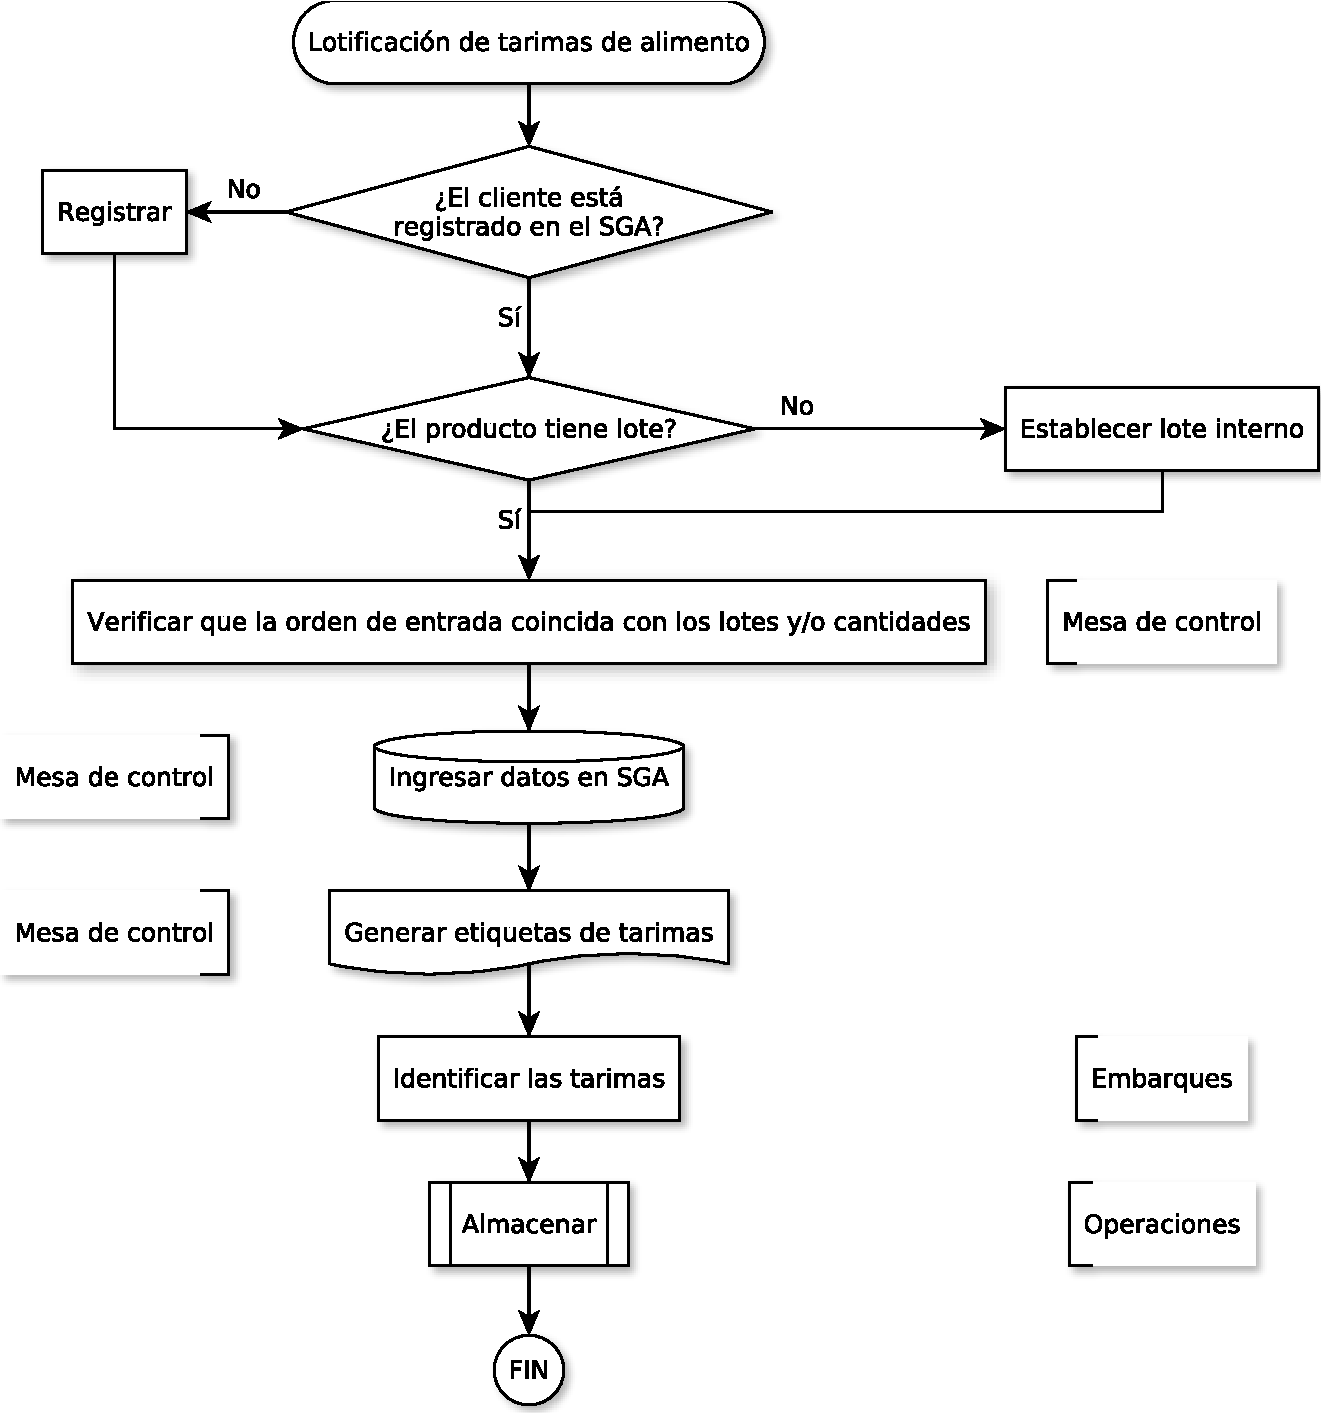
\includegraphics[width=0.9\linewidth,height=0.9\textheight,keepaspectratio]{../IT/IT-3 - Lotificación de tarimas.pdf}
    \caption[Proceso de lotificación de tarimas]{Proceso de lotificación de tarimas. Para mayor información, consultar el \cref{IT-3-LotificacionDeTarimas}.}
\end{scheme}

\begin{nota}{Identificadores de tarimas}{esp:IdTarimas}
    Las etiquetas para tarimas llevan la siguiente información:
        \begin{itemize}
            \item Fecha de recepción;
            \item nombre del cliente;
            \item nombre del alimento;
            \item fecha de caducidad;
            \item orden de compra o lote;
            \item numero de entrada;
            \item cantidad por tarima.
        \end{itemize}
\end{nota}

\Resp{\OP\ y \MC}{\AC}{\G} % Responsables

\AcPGen	% Acciones preventivas genericas

% \AcCGen	% Acciones correctivas genericas

\subsubsection{Acciones correctivas}
\begin{itemize}
\item En caso de no-conformidad, reportar en \mbox{formulario de {\slshape \RAC.}}
\end{itemize}

\subsection{Frecuencia}
\begin{itemize}
	\item Cada recepción de alimento;
	\item Cada entrega de alimento.
\end{itemize}

\begin{changelog}[title=Registro de cambios,simple, sectioncmd=\subsection*,label=changelog-\thesection-\MayorVer.\MenorVer]

	\begin{version}[v=2.1, date=2023--01, author=Pablo E. Alanis]
		\item Cambio de formato;
		\item Cambios en la serialización de versiones;
	\end{version}

	\begin{version}[v=1.3, date=2022--05, author=Alonso M.]
		\item cambio de fecha;
		\item cambio de código.
	\end{version}

	\shortversion{v=1.2, date=2021--05, changes=No hubo cambios}
\end{changelog}